\documentclass{article}
\usepackage[T1]{fontenc}
\usepackage{lmodern}
\usepackage{graphicx}
\usepackage{amsmath,amssymb}
\usepackage[a4paper,margin=2cm]{geometry}
\usepackage[absolute,overlay]{textpos}
\setlength{\TPHorizModule}{1mm}
\setlength{\TPVertModule}{1mm}
\usepackage[indonesian]{babel}
\usepackage{hyperref}
\setlength{\emergencystretch}{2em}
% unit: Halaman 74

\begin{document}

% === Halaman 74 (llm) ===

Algoritma enkripsi:\
1. Jika dua huruf terdapat pada baris kunci yang sama maka tiap huruf diganti dengan huruf di kanannya (bersifat siklik).

\vspace{10mm}

\vspace{10mm}

Cipherteks: FK \hfill Cipherteks: RM

% deskripsi: Ilustrasi proses enkripsi bigram 'di' menggunakan tabel Playfair, di mana huruf 'd' dan 'i' berada di baris yang sama sehingga diganti oleh huruf di kanannya yaitu 'f' dan 'k'.
% bbox normalisasi: [0.0900, 0.3700, 0.3200, 0.8000]
\begin{textblock*}{48.30mm}(18.90mm,109.89mm)
\noindent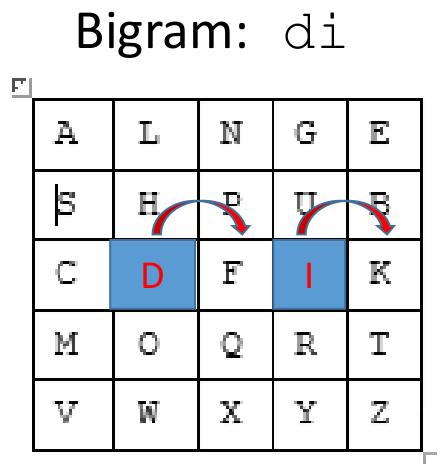
\includegraphics[width=48.30mm,height=127.71mm]{../../images/llm/page_074_img_01.png}%
\end{textblock*}

% deskripsi: Ilustrasi proses enkripsi bigram 'qt' menggunakan tabel Playfair, di mana huruf 'q' dan 't' berada di baris yang sama sehingga diganti oleh huruf di kanannya yaitu 'r' dan 'm' (siklik kembali ke awal baris).
% bbox normalisasi: [0.5700, 0.3700, 0.8200, 0.8000]
\begin{textblock*}{52.50mm}(119.70mm,109.89mm)
\noindent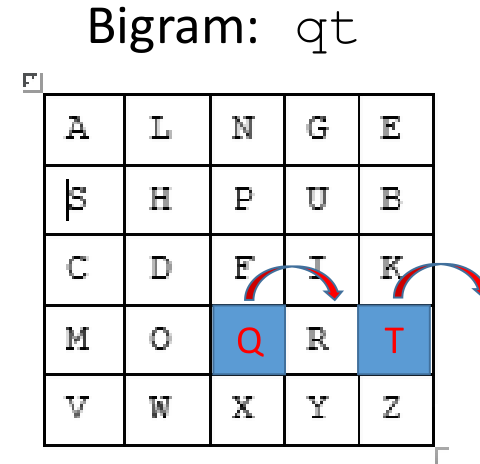
\includegraphics[width=52.50mm,height=127.71mm]{../../images/llm/page_074_img_02.png}%
\end{textblock*}

\end{document}
